\chapter{Neural Networks and Fourier Neural Operators}\label{ch:FNO+NN}
So far, we have studied numerical methods for solving partial differential equations (PDEs).
The finite volume method (FVM), along with other numerical solvers such as the finite difference method (FDM) and finite element method (FEM), solves PDEs by discretizing the domain into a grid.
A finer grid improves the accuracy of the solution but also increases the computational cost, creating a trade-off between accuracy and efficiency.
Complex PDEs often require a fine grid to accurately capture the solution, which can be computationally expensive.

In this chapter, we introduce the use of data-driven methods for solving PDEs.
%The hope of these methods is that they are able to reduce computational costs while maintaining high accuracy by learning the underlying dynamics of the solution.
%The primary goal of these methods is to reduce computational costs while preserving high accuracy by learning the underlying dynamics of the solution.
We will introduce the concepts of convolutional neural networks (CNNs) and Fourier neural operators (FNOs).

\section{Convolutional Neural Networks}
Convolutional neural networks (CNNs) are a specialized class of artificial neural networks designed to process and analyze data with a grid-like topology, such as images or time-series data represented by 2D grids.
CNNs excel at extracting spatial featues from data through the use of convolutional layers, which apply learnable filters to detect patterns such as edges, shapes or textures.
These layers are typically followed by pooling layers for dimensionality reduction and fully connected layers for classification or regression tasks.
A key advantage of CNNs is their ability to reduce the number of parameters compared to fully connected networks by sharing weights across spatial regions, making them computationally efficient and less prone to overfitting when working with large inputs.
Although CNNs are traditionally used for image recognition tasks, their architecture is adaptable for time-series analysis, especially when the data is structured spatially or sequentially.

In this project, CNNs are used to solve the shallow water equations, by training on the solution data generated by the FVM solver.
We aim to learn the underlying dynamics of the system by training the CNN on sequences of input-output pairs, where the input is the state of the system at time $t$ and the output is the state at time $t + \Delta t$.
The network is trained to construct a flow map. % which predicts the state of the system at the next time step based on sequences of input data.
The flow map $\Phi^t: \mathbb{R}^n \rightarrow \mathbb{R}^n$ is defined such that, for all $x \in X$ and all $t \in \mathbb{R}$:
\begin{align*}
    \Phi^t(x_0) =  x(t),
\end{align*}
where $x(t)$ is the solution of the PDEs with initial condition $x(0) = x_0$.
The flow map satisfies
\begin{align*}
    \Phi(\Phi (x, t), s) = \Phi(x, s + t),
\end{align*}
A CNN can approximate the flow map $\Phi$ by training on data that pairs an initial state $x_0$ with its state at later times $x(t)$.
The goal is to learn the mapping:
\begin{align*}
    x(t) = \Phi_{CNN} (x_0), 
\end{align*}
where $\Phi_{CNN}$ is the CNNS' approximation of the flow map.
The CNN model is trained on input-output pairs of sequences of data, with a sequence length of $N$.
\begin{align*}
    \begin{bmatrix}
        x_0 \\ x_1 \\ \vdots \\ x_{N-1}
    \end{bmatrix}
    \to
    \begin{bmatrix}
        x_1 \\ x_2 \\ \vdots \\ x_{N}
    \end{bmatrix}
\end{align*}


Meaning the network takes sequences of input data, and predicts the corresponding output data.
The output of the CNN is the solution at the next time step, effectively learning the dynamics of the SWE through the time-series data.
This setup allows the model to capture both spatial and temporal dependencies in the data, leveraging the CNN's ability to learn localized featires while processing sequential information.
A pro of CNN's is that they are efficient. By processing data in parallel using convolutional layers, the CNN efficiently handles large datasets without requiring excessive computational resources.
Another pro is the adaptability. 
The model's ability to learn from sequential data makes it adaptable for time-series predictions in dynamic systems like the shallow water equations.
A con is the data representation. Representing time-series data as sequences may require preprocessing, which can introduce complexity or a potential loss of information.
There can also be temporal limitations, as CNNs lack explicit mechanisms to model long-term temporal dependencies (unless extended with additional architechtures like RNNs or Transformers).
We will test and evaluate the performance of the CNN model in \autoref{ch:data-driven-results}.

%A classical neural network (NN) learns a mapping from input to output, i.e., a mapping between finite-dimensional spaces.
%Convolutional Neural Networks (CNNs) are a type of neural network that is particularly well-suited for image processing tasks.
%CNNs are designed to recognize patterns in spatial data, such as images, by using convolutional layers.
%A convolutional layer applies a set of filters to the input data, which allows the network to learn spatial hierarchies of patterns.
%The filters are learned during the training process, enabling the network to automatically extract features from the input data.
%CNNs have been widely used in image classification, object detection, and image segmentation tasks, among others.

%While CNNs have shown promise for solving PDEs, they have limitations when it comes to capturing long-range dependencies in the data.
%PDEs often involve interactions between distant points in the domain, which can be challenging for CNNs to capture.
%Another issue we are facing in this project is non-linearities.
%Standard neural networks uses combinations of linear multiplications and non-linear activation functions to approximate non-linear functions.



\section{Fourier Neural Operators}
In this section, we introduce the concept of Fourier Neural Operators (FNOs), a method for approximating mappings between infinite-dimensional function spaces.
The theory and method described here are based on the paper~\cite{FNO_2021}.
The goal is to learn a mapping between two infinite dimensional spaces from a finite collection of input-output pairs. 
Consider the operator $G: A \to U$, which maps from an infinite-dimensional function space $A$ to another infinite-dimensional function space $U$.
We aim to approximate the exact operator $G$ by constructing the map
\begin{align*}
    G_{\theta}: A \mapsto U, \quad \theta \in \Theta,
\end{align*} 
where $\Theta$ is a finite-dimensional parameter space.
Consider the functions $a \in A$ and $u \in U$.
We assume access to data in the form of pointwise evaluations of these functions, i.e., we have access to the observations ${\{a_j, u_j \}}_{j=0}^N$, in a domain $D \subset \mathbb{R}^d$, which is bounded open set.
The first step is to create $v_0(x) = P(a(x))$ by the input layer $P$, which is typically a shallow fully-connected neural network.
The neural operator is iterative, meaning we apply several iterations of updates to obtain $v_1, v_2, \ldots$ up to $v_T$.
An update $v_t \mapsto v_{t+1}$ is defined as
\begin{align}
    v_{t+1}(x) := \sigma \left( W v_t(x) + \left( \mathcal{K}(a;\phi)v_t \right) (x) \right), \quad \forall x \in D,
\end{align}
where $W: \mathbb{R}^{d_v} \to \mathbb{R}^{d_v}$ is a linear transformation, and $\sigma: \mathbb{R} \to \mathbb{R}$ is a non-linear activation function.
The output $u(x) = Q(v_T(x))$ is the final update $v_T$ transformed by the output layer $Q$.
There are various types of operators, but the core of the Fourier neural operator lies in its kernel function $\mathcal{K}$.
We define the Fourier integral operator $\mathcal{K}$ as 
\begin{align}
    \left( \mathcal{K}(\phi)v_t \right) (x) := \mathcal{F}^{-1} \left( R_{\phi} \cdot (\mathcal{F}v_t ) \right)(x), \quad \forall x \in D,
\end{align}
where $\mathcal{F}$ is the Fourier transform, $\mathcal{F}^{-1}$ is the inverse Fourier transform, and $R$ is the linear transformation applied on the lower Fourier modes. 
By transforming the data into the Fourier domain, FNOs can take advantage of the periodicity and smoothness properties of the Fourier basis, which simplifies the learning process for functions defined over continuous domains.
This approach leverages the fact that differentiation with respect to time is equivalent to multiplication in the Fourier domain, distinct from the convolution theorem. CITE.
The network architechture for the FNO model is illustrated in \autoref{fig:fourier_neural_network}.
\begin{figure}[H]
    \centering
    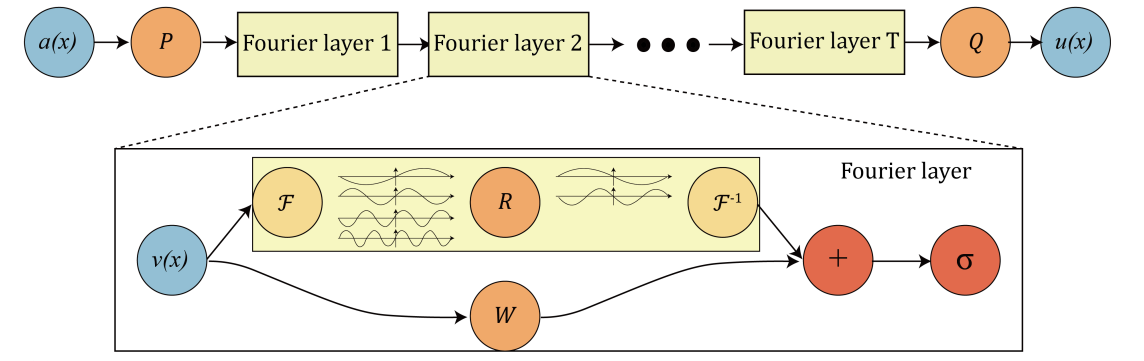
\includegraphics[width=0.7\textwidth]{C:/Users/Matteo/Shallow-Water-Equations/figs/fourier_neural_network.png}
    \caption{An overview of the network architecture with several Fourier layers. Illustration from~\cite{FNO_2021}.
            Top: Overall structure with input function $a$, input layer $P$, several Fourier layers, output layer $Q$ and output function $u$.\\
            Bottom: A Fourier layer consists of two parallel paths. Top is a Fourier transformation $\mathcal{F}$, a linear transformation $R$ and an inverse Fourier transformation $\mathcal{F}^{-1}$.
            The bottom path consists of a linear transformation $W$. The parts meet and undertake an activation function $\sigma$.}\label{fig:fourier_neural_network}
\end{figure}
From the top in \autoref{fig:fourier_neural_network} we see that the network consists of an input function $a(x)$, an input layer $P$, several Fourier layers, an output layer $Q$ and some output function $u(x)$.
As we only have access to pointwise evaluations of $a(x)$ and $u(x)$ these are what we will use. 
That is, our goal is to approximate the input-output mapping: 
\begin{align*}
    \begin{bmatrix}
        a_0 \\
        a_1 \\
        \vdots \\
        a_{N-1}
    \end{bmatrix}
    \to
    \begin{bmatrix}
        u_0 \\
        u_1 \\
        \vdots \\
        u_{N-1}
    \end{bmatrix}.
\end{align*}
In the context of this project we have that $a(x) = v_t(x)$ and $u(x) = v_{t+1}(x)$.

In the bottom of \autoref{fig:fourier_neural_network} we see the structure of a Fourier layer, which consists of two parallel paths.
In the top path, the data undergoes a Fourier transform $\mathcal{F}$, decomposing it into a sum of Fourier basis functions (sines and cosines) with varying frequencies, amplitudes and phases.
A linear transformation $R$ it the applied to filter out the higher Fourier modes, as illustrated in the figure, where high-frequency components are removed.
When implementing the model, we choose the number of Fourier modes to retain, depending on how much information we want to preserve.
Retaining more modes keeps more information, but may also introduce more noise and oscillations.
After filtering, the inverse Fourier transform $\mathcal{F}^{-1}$ is applied to reconstruct the data in its original form.
The bottom path involves a linear transformation $W$, and the two paths merge before applying a non-linear activation function $\sigma$.

A key advantage of FNOs is that since they learn mapping between function spaces, they are not constrained by a specific grid or mesh.
This allows them to transfor solutions across different grids, a process known as zero-show super-resolution.
The learned operator can generalize from the coarse grid to the fine grid without needing to be retrained, making it grid-independent.
This is a major advantage because it reduces the computational cost associated with fine-grid simulations.
In \autoref{ch:data-driven-results}, we will evaluate the performance of the implemented FNO model in this context, testing its ability to maintain high accuracy when making predictions on finer grids.

\subsection*{Multistep prediction}
We aim to develop a multi-step prediction model that can predict a specified number of time steps ahead.
The input-output pairs are given as $\{a_j, u_j\}_{j=0}^N$, where the points $\{u\}_{j=0}^N$ represent the values one time step after $\{a\}_{j=0}^N$.
We collect state pairs $\{v_t, v_{t+1}\}_{j=0}^N$ for training a flowmap.
Feeding this data into the model allows it to learn the flow map for the system.
We are dealing with time series data, and the original form of the FNO can predict one time step ahead.
However, for many applications, predicting multiple time steps ahead is more useful.
To enable multi-step predictions, we organize the input data into sequences.
The model is trained to predict the output state based on data from several previous time steps, with a specified sequence length.
That is, the input data is given as
\begin{align*}
    \{v_{t-n}, v_{t-n+1}, \dots, v_{t+1}\}_{j=0}^N,
\end{align*}
where $n$ is the sequence length.

We will conduct experiments to determine the optimal sequence length for our model.

During prediction, the model's output is added to the input as the newest data point, replacing the oldest data.
This process is repeated until predictions for the desired number of future time steps are made.
The process is illustrated in \autoref{fig:multistep_pred_flowchart}.
\begin{figure}[H]
    \centering
    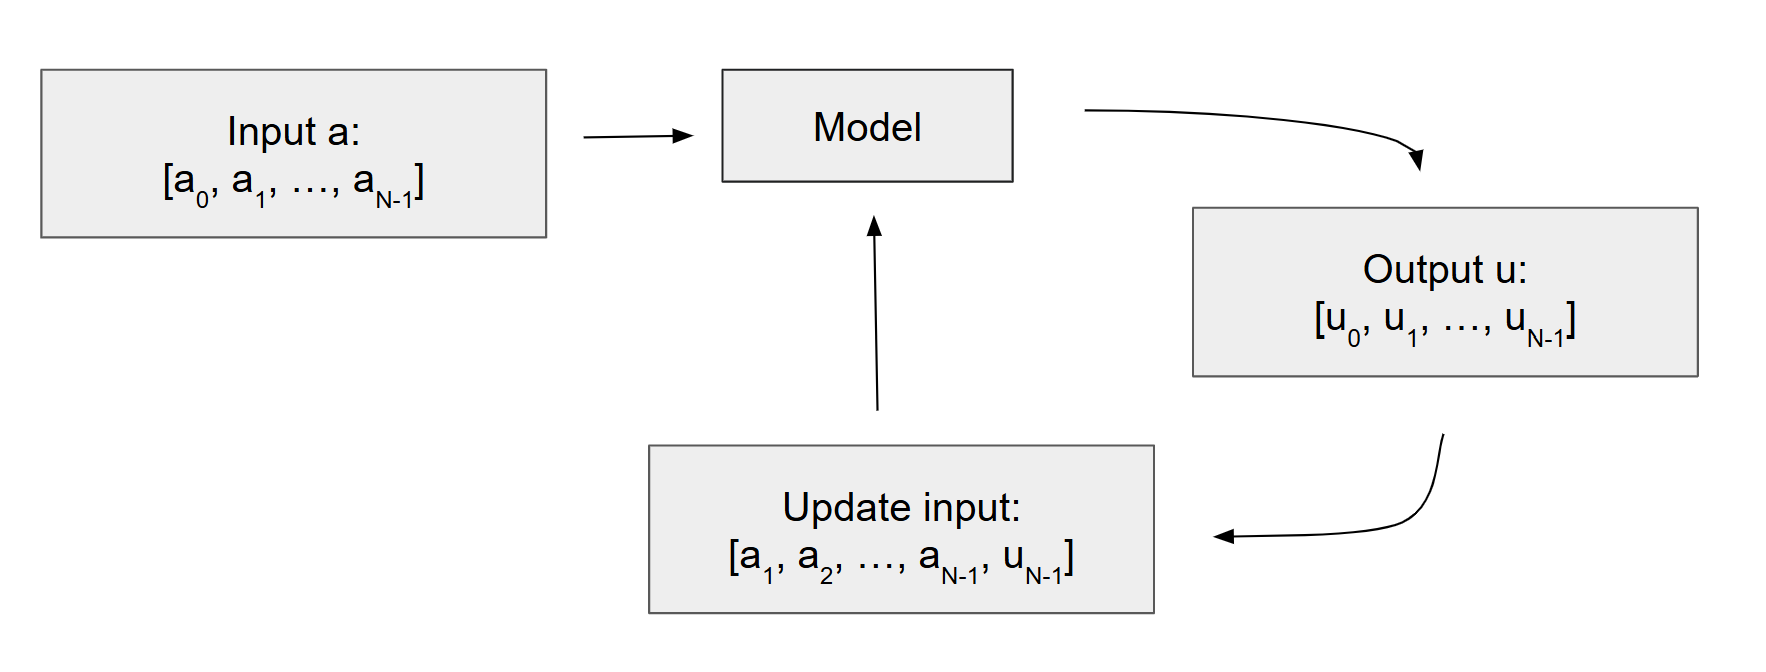
\includegraphics[width=0.7\textwidth]{C:/Users/Matteo/Shallow-Water-Equations/figs/multistep_pred_flowchart.png}
    \caption{Flowchart of the multi-step prediction process.}\label{fig:multistep_pred_flowchart}
\end{figure}
The results of the multi-step prediction model will be presented in \autoref{ch:data-driven-results}.



%Another issue we are facing in this project is non-linearities.
%Whereas, neural operators approximate non-linear operators, by combining linear functions and non-linear activation functions with global integral operators. 

%Both methods require only data, not the PDE itself, which is a significant advantage when the governing PDE is unknown.
